\documentclass[main.tex]{subfiles}

\begin{document}

\section*{Goal}
Today we will investigate the angular counterparts to force and momentum, torque and angular momentum respectively. In our experiment on torque we will see how the placement of the applied force can affect the torque on an object. Then, in our angular momentum experiment we will use the conservation of angular momentum to calculate the moment of inertia of several different objects.

\section*{Equipment}
\begin{itemize}
\item
Pegboard levers
\item
Masses
\item
Meter stick
\item
String
\item
Support frame
\item
Torque problem at lecture table
\item
Rotary Motion Sensor
\item
Silver Disk, White Disk, Rod with masses, Odd-Shaped Object
\item
Triple-beam Balance
\end{itemize}•

\section*{Theory}
\subsection*{Torque}

\begin{wrapfigure}{r}{0.5\textwidth}
\centering
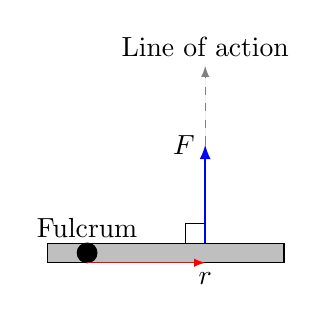
\begin{tikzpicture}[
	force/.style={thick,>=latex,draw=blue,fill=blue},
	axis/.style={dashed,>=latex,draw=gray,fill=gray},
	radial/.style={>=latex,draw=red,fill=red}
]
%\draw[help lines] (0,0) grid (3,3);
	\draw[fill=lightgray] (0,0) rectangle (3,0.25);
	\draw[fill=black] (0.5,0.125) circle [radius=0.125] node [above,yshift=2pt] {Fulcrum};
	
	\draw[force,->] (2,0.25) -- (2,1.5) node [left] {$F$};
	\draw[axis,->] (2,1.5) -- (2,2.5) node [above] {Line of action};
	\draw[radial,->] (0.5,0) -- (2,0) node [below] {$r$};
	
	\draw (1.75,0.25) -- (1.75,0.5) -- (2,0.5);
\end{tikzpicture}
\caption{} \label{fig:Torque}
\end{wrapfigure} \vspace{-10pt}

When we apply a force on an elongated object a distance $r$ from some point of rotation we will create a torque on the object. As in Figure~\ref{fig:Torque} the point that the body rotates around is called the fulcrum. The force $F$ on the object is applied along a line we call the ``Line of action." The distance $r$ is called the lever arm which is always measured \emph{from} the fulcrum \emph{to} the line of action of the force. In general the torque vector of the force with respect to the fulcrum is defined as,
\begin{equation} \label{eq:VectTorque}
\boldsymbol{\tau}=\mathbf{r} \times \mathbf{F},
\end{equation}
where this is the vector product of the vectors $\mathbf{r}$ and $\mathbf{F}.$ One of the properties of vector products is that the resultant must always be \emph{orthogonal} or mutually perpendicular to both parent vectors, so we can handle the direction and magnitude of our torque separately. The magnitude of torque is,
\begin{equation} \label{eq:MagTorque}
\tau=rF\sin\theta,
\end{equation}
where $\theta$ is the angle between the vectors $\mathbf{r}$ and $\mathbf{F}.$ For most of our experiment $\theta=\pi/2$ so Equation~\eqref{eq:MagTorque} simplifies to,
\begin{equation}
\tau=rF.
\end{equation}

To determine the direction of the torque we use what is known as the ``right-hand rule." This simple mnemonic is true for all vector products and is setup as follows: The index finger of the right hand is pointed in the direction of the first vector of the product ($\mathbf{r}$), the middle finger is pointed in the direction of the second vector ($\mathbf{F}$), then the thumb will be pointing in the correct direction of the resultant vector ($\boldsymbol{\tau}$).
% Try to find an image of the Right-Hand Rule

Finally, for a body that is in translational and rotational equilibrium, meaning that the the sums of the forces and the torques are both zero, the point that we choose for the fulcrum is arbitrary. We can choose any point on the body and the sum of the torques will still be zero. This is extremely advantageous for us because we can then choose a fulcrum that makes our calculations easier.

\subsection*{Angular Momentum}
The last rotational quantity we want to investigate in this class is angular momentum. As can be assumed angular momentum $\mathbf{L}$ is related to linear momentum $\mathbf{p}$ in the same way that torque is related to force,
\begin{equation} \label{eq:VectAngMom}
\mathbf{L}=\mathbf{r} \times \mathbf{p}.
\end{equation}
As it was with Equation~\eqref{eq:MagTorque} the magnitude of angular momentum is,
\begin{equation}\label{eq:MagAngMom}
L=rp\sin\theta,
\end{equation}
and if $\theta=\pi/2$ then Equation~\eqref{eq:MagAngMom} simplifies to 
\begin{equation} \label{eq:Lmvr}
L=rp=mvr
\end{equation}
We can however write an expression completely in terms of angular quantities which will be more useful to us given our equipment. Let us consider our body as a collection of small pieces. Each piece of mass $m_i$ will rotate around a circle centered on the axis of rotation with a velocity $v_i.$ This tangential velocity vector $\mathbf{v}_i$ will always be perpendicular to a position vector $\mathbf{r}_i$ as we saw last chapter. We also know from the previous chapter that $v_i=r_i\omega.$ Therefore we can write Equation~\eqref{eq:Lmvr} as,
\begin{equation}
L_i=m_i(r_i\omega)r_i=m_ir_i^2\omega.
\end{equation}
Now the total angular momentum $L$ of the body will be the sum of all the individual angular momenta $L_i$ of the particles,
\begin{equation}
L=\sum L_i=\left(\sum m_ir_i^2\right)\omega=I\omega,
\end{equation}
where we define $I=\sum m_ir_i^2$ to be the moment of inertia of the body and describes how mass is distributed around a rotating body. 
\begin{table}
\begin{tabular}{|p{0.3\textwidth}|c|c|}
\hline
\textbf{Point Mass} (at a distance $r$ from the axis of rotation) & 
\raisebox{-0.6\height}{
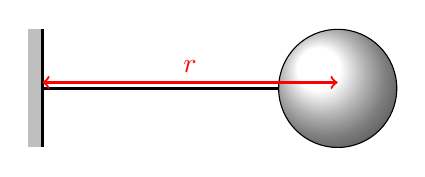
\begin{tikzpicture}[scale=0.75]
	\fill[ball color=white!10] (0,0) circle (1cm);
	\draw (0,0) circle (1cm);
	\draw[very thick] (-1,0) -- (-5,0);
	\fill[color=lightgray] (-5,1) --(-5,-1) -- (-5.25,-1) -- (-5.25,1) -- cycle;
	\draw[very thick] (-5,1) -- (-5,-1);
	\draw[<->,red,thick] (0,0.1) -- (-5,0.1) node [midway, above] {$r$};
\end{tikzpicture}
}
& $I=mr^2$\\
\hline
\textbf{Solid Disk} (of radius $r$ rotating about an axis through the center of the disk) &
\raisebox{-0.7\height}{
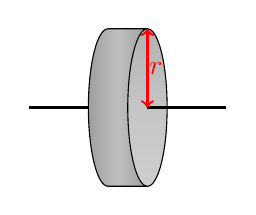
\begin{tikzpicture}[scale=0.5,rotate=-90]
	\fill[left color=gray!50!black,right color=gray!50!black,middle color=gray!50,shading=axis,opacity=0.25] (2,0) -- (2,1) arc (360:180:2cm and 0.5cm) -- (-2,0) arc (180:360:2cm and 0.5cm);
	\fill[top color=gray!90!,bottom color=gray!2,middle color=gray!30,shading=axis,opacity=0.25] (0,1) circle (2cm and 0.5cm);
	\draw (-2,1) -- (-2,0) arc (180:360:2cm and 0.5cm) -- (2,1) ++ (-2,0) circle (2cm and 0.5cm);
	\draw[very thick] (0,-2) -- (0,-0.5);
	\draw[very thick] (0,1) -- (0,3);
	\draw[<->,red,thick] (0,1) -- (-2,1) node [midway,right,xshift=-3pt] {$r$};
\end{tikzpicture}
}
& $I=\frac{1}{2}mr^2$\\
\hline
\textbf{Thin Rod} (of length $l$ rotating about an axis perpendicular to the rod and through its center) &
\raisebox{-0.8\height}{
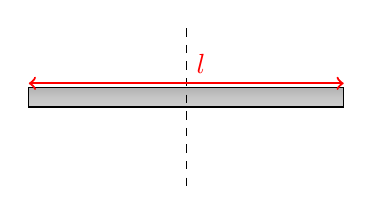
\begin{tikzpicture}[scale=1]
	\fill[top color=gray!90!,bottom color=gray!2,middle color=gray!30,shading=axis,opacity=0.25] (-2,0) rectangle (2,0.25);
	\draw (-2,0) rectangle (2,0.25);
	\draw[dashed] (0,1) -- (0,-1);
	\draw[<->,red,thick] (-2,0.3) -- (2,0.3) node [midway, above right] {$l$};
\end{tikzpicture}
}
& $I=\frac{1}{12}ml^2$\\
\hline
\end{tabular}•
\caption{} \label{tab:I_obj}
\end{table}
Table~\ref{tab:I_obj} provides the formulas of the various geometries that we will use in our experiment. An important property about moments of inertia is that it is an additive quantity, meaning that if two or more objects are combined into one compound object then then total moment of inertia will be the sum of the individual moments.
\[
\sum I=I_1+I_2+\dotsb
\]
The \emph{conservation of angular momentum} states that in the absence of a net external torque, the total angular momentum of the system is constant. In our experiment we will be colliding two objects together. One object will always be the silver disk that is attached to the Rotary Motion Sensor. We will begin each collision by spinning the silver disk . Then we will drop onto it the second object, which will initially have zero angular velocity. All of our collisions will be perfectly inelastic collisions, meaning that the objects will stick together and rotate with the same final angular velocity. Thus,
\begin{align}
L_i&=L_f \nonumber\\
I_1\omega_i &= (I_1+I_2)\omega_f. \label{eq:ConsAngMom}
\end{align}•

\section{Setup I: Torque}
\subsection*{Procedure}
\begin{enumerate}
\item
Support the pegboard lever at the center by hanging it on a string attached to a hook ring. Verify that the board is approximately balanced in horizontal position at that point.
\item
Attach a 200 g mass to the third hole from the center using the lower line of holes. Calculate the mass needed at the sixth hole from the center on the opposite side to again balance the board. Hang that mass from the board and test for balance. Remember that there are uncertainties involved and make a list of their causes.
\item
Remove the last mass added and calculate what mass must be added at the fourth hole from the center on the side opposite the 200 g mass to re-balance the board. After testing the result, derive a simple formula that works for any situation.
\item \label{step:LeverBoard_start}
Remove all added masses and move the supporting string to the sixth hole from the center on the top row of holes. Add enough mass at the eighth hole on the same side to balance the lever board. Recall that the weight of the board can be approximated to a point at the center, use the formula derived in the previous step to determine  the mass of the board.
\item \label{step:LeverBoard_end}
Use the triple-beam balance to measure the mass of the lever board.
\item
At the lecture desk is a rod and ball setup that is in rotational equilibrium. Record the scale values (in the proper units) and angles of the supporting strings using the protractor available. Make all length measurements deemed necessary to determine the mass of the bar and the mass of the ball hanging from the bar. Assume the center of the mass of the bar is at the center of the bar.
\end{enumerate}•

\subsection*{Analysis}
\begin{enumerate}
\item
Determine the relative discrepancy in the mass of the lever board by comparing the results from steps~\ref{step:LeverBoard_start}--\ref{step:LeverBoard_end}.
\item
Determine the mass of the bar and the ball hanging from the bar.
\end{enumerate}•

\section{Setup II: Angular Momentum}
For this setup, we will use the Rotary Motion Sensor (RMS) to measure the angular velocity of our system before and after we drop an object on the rotating silver disk.
\begin{enumerate}
\item
Open Capstone.
\item
Connect the RMS to the 850UI then setup Capstone to record from the sensor (click on the left-most port that the sensor is plugged into).
\item
Create a graph of Angular Velocity vs Time.
\item
Mount the RMS on the vertical rod in the table so that the disks will be on top.
\end{enumerate}•

\subsection*{Procedure}
\begin{enumerate}
\item
Measure the mass of the silver disk and record it. Measure the diameter of the silver disk three different times from different locations on the disk and record the average.
\item
Attach the silver disk to the RMS.
\item \label{step:AngMom_start}
Measure the mass of the white disk and record it. Measure the diameter three different times from different locations on the disk and record the average.
\item
Give the silver disk a spin. Click on the Record button to start data collection. After about 25 data points have been recorded, drop the white disk onto the spinning disk. After the collision click the Stop button to end the data collection. Rescale the data. If the collision on the graph is not sharp enough, then delete the data run and repeat this step.
\item \label{step:AngMom_end}
Click on the Coordinates Tool 
\includegraphics{Coordinates_Tool} and move it to the data point immediately before the collision. Record the angular velocity at this point in the data table as the initial angular velocity. Now move the tool to the data point immediately after the collision. Record the angular velocity at this point as the final angular velocity.
\item
Repeat steps~\ref{step:AngMom_start}--\ref{step:AngMom_end} with the silver disk and the rod. For the rod we will need to measure its mass (without the attached masses) and overall length, the mass of each attachable mass removed from the rod and the distance of each attachable mass from the center of rotation. Make sure the masses are attached at the outer set of holes.
\item
Repeat steps~\ref{step:AngMom_start}--\ref{step:AngMom_end} with the silver disk and the odd-shaped object. We only need to measure the mass of this object.
\item
Show all data runs with the Select Data Run button 
\includegraphics{Select_Data_Run}. \textbf{Print} out a copy of this graph for each group member.
\item[\emph{Optional:}]
Repeat steps~\ref{step:AngMom_start}--\ref{step:AngMom_end} with the silver disk and the rod. This time, move the masses to the inner set of holes on the rod. \textbf{Print} a copy of this run for each group member.
\end{enumerate}•

\subsection*{Analysis}
\begin{enumerate}
\item
We will use the white disk run to determine an experimental value for the moment of inertia of the silver disk and compare it to a theoretical value.
\begin{enumerate}
\item
Using the appropriate formula from Table~\ref{tab:I_obj}, calculate the theoretical moments of inertia for both disks.
\item
Using Equation~\eqref{eq:ConsAngMom} with the measured angular velocities and the theoretical moment of inertia for the \emph{white} disk calculate the moment of inertia for the \emph{silver} disk.
\item
Calculate the percent discrepancy of the experimental value for the moment of inertia of the silver disk with its theoretical value.
\end{enumerate}•
\item \label{step:Rod}
For the the rod/masses run we will determine an experimental value of the moment of inertia of the rod with attached masses and compare it to a theoretical value.
\begin{enumerate}
\item
To determine the theoretical moment of inertia of the rod with attached masses, we must first calculate the individual moments of inertia for each piece using the appropriate formulas from Table~\ref{tab:I_obj}. (We can treat the attachable masses as point masses.) Calculate the total moment of inertia by  summing each individual moment together.
\item
Using Equation~\eqref{eq:ConsAngMom} with the measured angular velocities and the \emph{experimental} moment of inertia for the silver disk, calculate the moment of inertia for the rod/masses.
\item
Calculate the percent discrepancy of the experimental moment of inertia of the rod/masses with its theoretical value.
\end{enumerate}•
\item
For the odd-shaped object run we will determine an experimental value for the moment of inertia for the object. We will then use this value to determine the \emph{radius of gyration}. If we consider revolving off center a point mass of the same mass as our object and with the same moment of inertia then the radius of gyration $r_G$ is given by,
\begin{equation} \label{eq:R_G}
I_{odd}=mr_G^2
\end{equation}
\begin{enumerate}
\item
Using Equation~\eqref{eq:ConsAngMom} with the measured angular velocities and the experimental moment of inertia of the silver disk, calculate the moment of inertia of the odd-shaped object.
\item
Using Equation~\eqref{eq:R_G} with the moment of inertia calculated in the previous step, determine the radius of gyration of the odd-shaped object.
\end{enumerate}•
\item[\emph{Optional:}]
For the optional rod/masses data, repeat analysis step~\ref{step:Rod}.
\end{enumerate}

\begin{question}
Why is it better to use the experimental value for the moment of inertia of the silver disk rather than the theoretical value? (Hint: What is not being considered in the theoretical formula?)
\end{question}
\begin{question}
The rotational kinetic energy is given by $KE=\frac{1}{2}I\omega^2.$ Is energy conserved in these three runs? Explain your answer.
\end{question}
\begin{question}[\emph{Optional}]
How is th moment of inertia with the attached masses changed by moving the masses to the inner holes? How should the final angular velocity change by moving the masses inwards?
\end{question}

\begin{samepage}
\hrulefill \\
\emph{Week Nine:} \textbf{Torque \& Angular Momentum}
\begin{enumerate}
\item
\textbf{(1)} Title Page
\item
\textbf{(39)} \emph{Angular Momentum}
\begin{enumerate}
\item
\textbf{(5)} Theory
\item
\textbf{(5)} Procedure
\item
\textbf{(1)} Graph with all three mandatory runs displayed.
\item
\textbf{(5)} Data Sheet
\item
\textbf{(14)} Data Analysis with sample calculations shown.
\item
\textbf{(4)} Answers to the mandatory questions.
\item
\textbf{(5)} Conclusion
\end{enumerate}•
\item
\textbf{(10)} \emph{Torque}
\begin{enumerate}
\item
\textbf{(5)} Data Sheet
\item
\textbf{(5)} Data Analysis with sample calculations shown.
\end{enumerate}•
\end{enumerate}•
\end{samepage}

\newpage
\begin{doublespace}
\section{Data Sheets}
\subsection*{Torque}
Mass needed to counter 200 g at third hole:\rule[-1mm]{2.5cm}{.1pt}\\
Uncertainties: \\[3cm]
Mass needed to counter 200 g at fourth hole:\rule[-1mm]{2.5cm}{.1pt}\\
Formula:\\[3cm]
Mass needed to counter weight of the board:\rule[-1mm]{2.5cm}{.1pt}\\
Mass of board (calculated):\rule[-1mm]{2.5cm}{.1pt}\\
Mass of board (measured):\rule[-1mm]{2.5cm}{.1pt}\\[1cm]
Lecture Desk Problem:\\
Force on string:\rule[-1mm]{2.5cm}{.1pt}, Angle:\rule[-1mm]{2.5cm}{.1pt}\\
Force on string:\rule[-1mm]{2.5cm}{.1pt}, Angle:\rule[-1mm]{2.5cm}{.1pt}\\
Sketch with lengths indicated:

\newpage
\subsection*{Angular Momentum}
Mass of Silver Disk:\rule[-1mm]{2.5cm}{.1pt}\\
Average Diameter of Silver Disk:\rule[-1mm]{2.5cm}{.1pt}\\ \\
Mass of White Disk:\rule[-1mm]{2.5cm}{.1pt}\\
Average Diameter of White Disk:\rule[-1mm]{2.5cm}{.1pt}\\ \\
Mass of Rod:\rule[-1mm]{2.5cm}{.1pt}\\
Length of Rod:\rule[-1mm]{2.5cm}{.1pt}\\ 
Mass of Attachable Mass 1:\rule[-1mm]{2.5cm}{.1pt} \qquad Mass of Attachable Mass 2:\rule[-1mm]{2.5cm}{.1pt}\\
Distance from center of rotation to attachable masses:\rule[-1mm]{2.5cm}{.1pt}\\ \\
Mass of Odd-Shaped Object:\rule[-1mm]{2.5cm}{.1pt}\\ \\
\emph{(Optional)} Distance from center of rotation to attachable masses:\rule[-1mm]{2.5cm}{.1pt}\\ \\

\begin{tabular}{|l|l|l|}
\hline
Object & $\omega_i$ (rad/s) & $\omega_f$ (rad/s)\\
\hline
White Disk &&\\
\hline
Rod with Masses &&\\
\hline
Odd-Shaped Object &&\\
\hline
\emph{Rod with Masses (Optional)} &&\\
\hline
\end{tabular}•
\end{doublespace}

\end{document}
